\subsection*{b)}
Wie ist es aufgebaut?

\section*{Antwort}
Ein Qualitätssystem ist hierarchisch aufgebaut und definiert ``Qualität`` durch \textbf{Qualitätsmerkmale} (\textit{QM}), die durch \textbf{Qualitätsteilmerkmale} (\textit{QTM}) konkretisiert werden.\\
Qualitätsteilmerkmale werden wiederum durch \textbf{Qqalitätsindikatoren} definiert, die messbare Eigenschaften repräsentieren: Dies erlaubt eine nominelle Bestimmung von Qualität in dem verwendeten Qualitätssystem (s. Abbildung~\ref{fig:qualitätssysteme}).

\begin{figure}
    \centering
    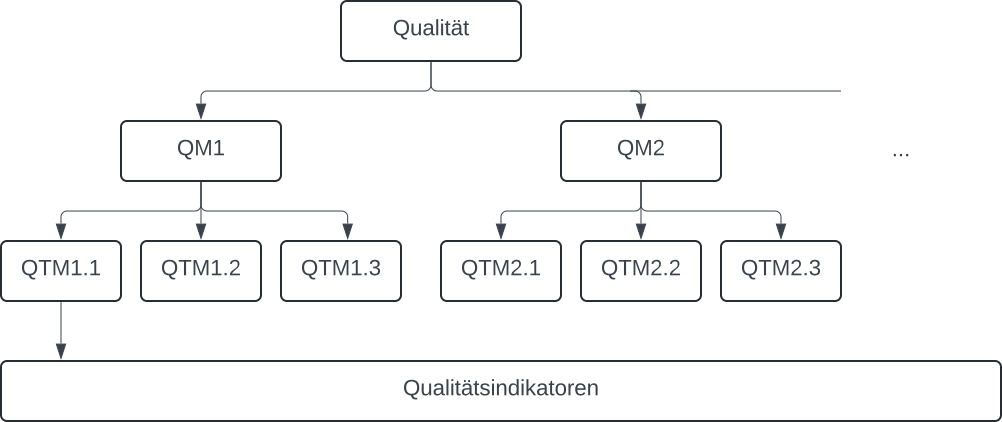
\includegraphics[scale=0.8]{chapters/aufgabe 1/img/qualitätssysteme}
    \caption{Skizzenhafter Aufbau von Qualitätssystemen. \textit{Qualitätsindikatoren} sind als breiter Balken dargestellt, da sich mehrere \textit{Qualitätsteilmerkmale} auf einen gemeinsamen \textit{Qualitätsindikator} beziehen können. (Quelle: in Anlehnung an~\cite[Abb. 1.1, 3]{Wed09c})}
    \label{fig:qualitätssysteme}
\end{figure}
